\chapter{Recommender Systems}
\label{theory}
\thispagestyle{plain}

Very often, users do not know the touristic points they would like to visit, the overwhelming amount of data requires mechanisms for efficient information filtering. The aim of the recommender system is to find sights that might interest users based on their past visits, and provide them with more relevant content.\\
\\
In this Chapter, we introduce some background concept about Recommender Systems~(RS) and their two different implementation approaches. In the following Sections, we describe the main goals of the recommender system and how it is used in our problem. We end up by justifying a chosen algorithm type for our recommender system implementation.

\section{Introduction}
\label{sec:theRecommenderSystem} 
\gls{rs} are used to generate meaningful information to a collection of users for items or products that might interest them. Nowadays, they are widely used, for example in electronic commerce company Amazon~\cite{AmazonRecommendGLBSJY}, which recommends additional items of what other shoppers bought along with the currently selected item. For instance, the Spotify~\cite{spotifyRecommenderEngine} music service implements the \gls{rs} which suggests new music to users based on their taste. There are many other services using this approach, because it makes easier the discovery of meaningful information without any additional effort by the user~\cite{recommSystemPMVS}. In our case, items are the points of interest to be recommended to users based on their past visits. Figure~\ref{fig:recomenderAlgoirthms} depicts different approaches and algorithm types of \gls{rs}.\\
%%%%%%%%%%%%%%%%%%%%%
\begin{figure}[h!]
 \centering
   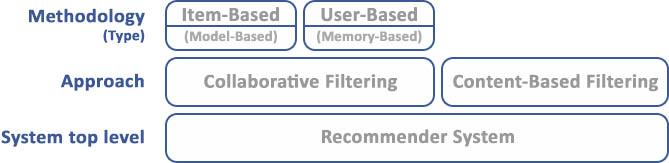
\includegraphics[width=10cm]{./images/flows/flow_recomender_hierarchy.jpg}
   \caption{Recommender systems hierarchy.}
   \label{fig:recomenderAlgoirthms}
\end{figure}
%%%%%%%%%%%%%%%%%%%%%
\\
The recommendation process can be done through the analysis of the items characteristics, named this as Content-Based Filtering (CBF). Another approach, designated as Collaborative Filtering (CF), consists in the collaboration between different users, and is divided into two main categories:
\begin{itemize}
\item \gls{ubcf} is used with memory-based type of algorithms. Consists in using user's rating in order to compute recommendations.
\item Item-Based Collaborative Filtering (IBCF) uses a model-based methodology. These type of \gls{rs} are developed using the data mining algorithms to find patterns based on training data.
\end{itemize}
In the following Sections, we describe each of these approaches, providing a comparative analysis.\\
\\
Table~\ref{tab:frequentSymbols} lists the symbols associated to \gls{cf} and \gls{cbf} terminology. 
\begin{table}[h]
\caption{List of frequently used symbols.}
\centering
\begin{tabular}{C{2.0cm} L{8cm}}
\hline\hline
Symbol&\multicolumn{1}{l}{Designation} \\
\hline
$I$ & A collection of $n$ items $\{i_{1}, i_{2}, \dots, i_{n}\}$\\
$U$ & A set of $m$ users $\{u_{1}, u_{2}, \dots, u_{m}\}$\\
$u_{a}$ & An active user\\
$I_{u_{a}}$ & A set of items that belong to $u_{a}$\\
~&~\\
$SIM$ & The similarity matrix of the items\\
$sim_{i,j}$ & Similarity between two distinct items $i$ and $j$\\
$P_{u,i}$ & Prediction for user $u$ and item $i$\\
~&~\\
$\bar{R}_{u}$ & The average of the $u$-th user's ratings\\
${R}_{u,i}$ & The rating value for item $i$ rated by user $u$\\
\hline
\end{tabular}
\label{tab:frequentSymbols}
\end{table}

\section{Overview of Content-based Filtering}
\label{sec:oftcbf}
\gls{cbf} methods are based on the information about the characteristics of the items to be recommended. These systems can evolve and learn user preferences from user's actions, but they are limited to recommend content of the same type as that the user is already using. In order to have an accurate recommender system with this kind of algorithms, the item should have a large set of characteristics associated to it, in order to establish a degree of similarity between two different items. 
As presented in Figure~\ref{fig:itemBasedProcess}, the input data of the algorithm is a vector
of items $I = \{i_{1}, i_{2}, \dots,  i_{n}\}$. The similarity computation is made between distinct pairs of values of the vector which then produces a similarity matrix filled with values representing
degrees of similarity $SIM = \{sim(i_{1},i_{2}), sim(i_{1}, {\dots}), \dots , sim(i_{2},i_{3}), \dots, sim(i_{n-1},i_{n})\}$ between each pair.
Finally, the recommendation process selects the top results as suggested items.\\
\\
\begin{figure}[h!]
 \centering
   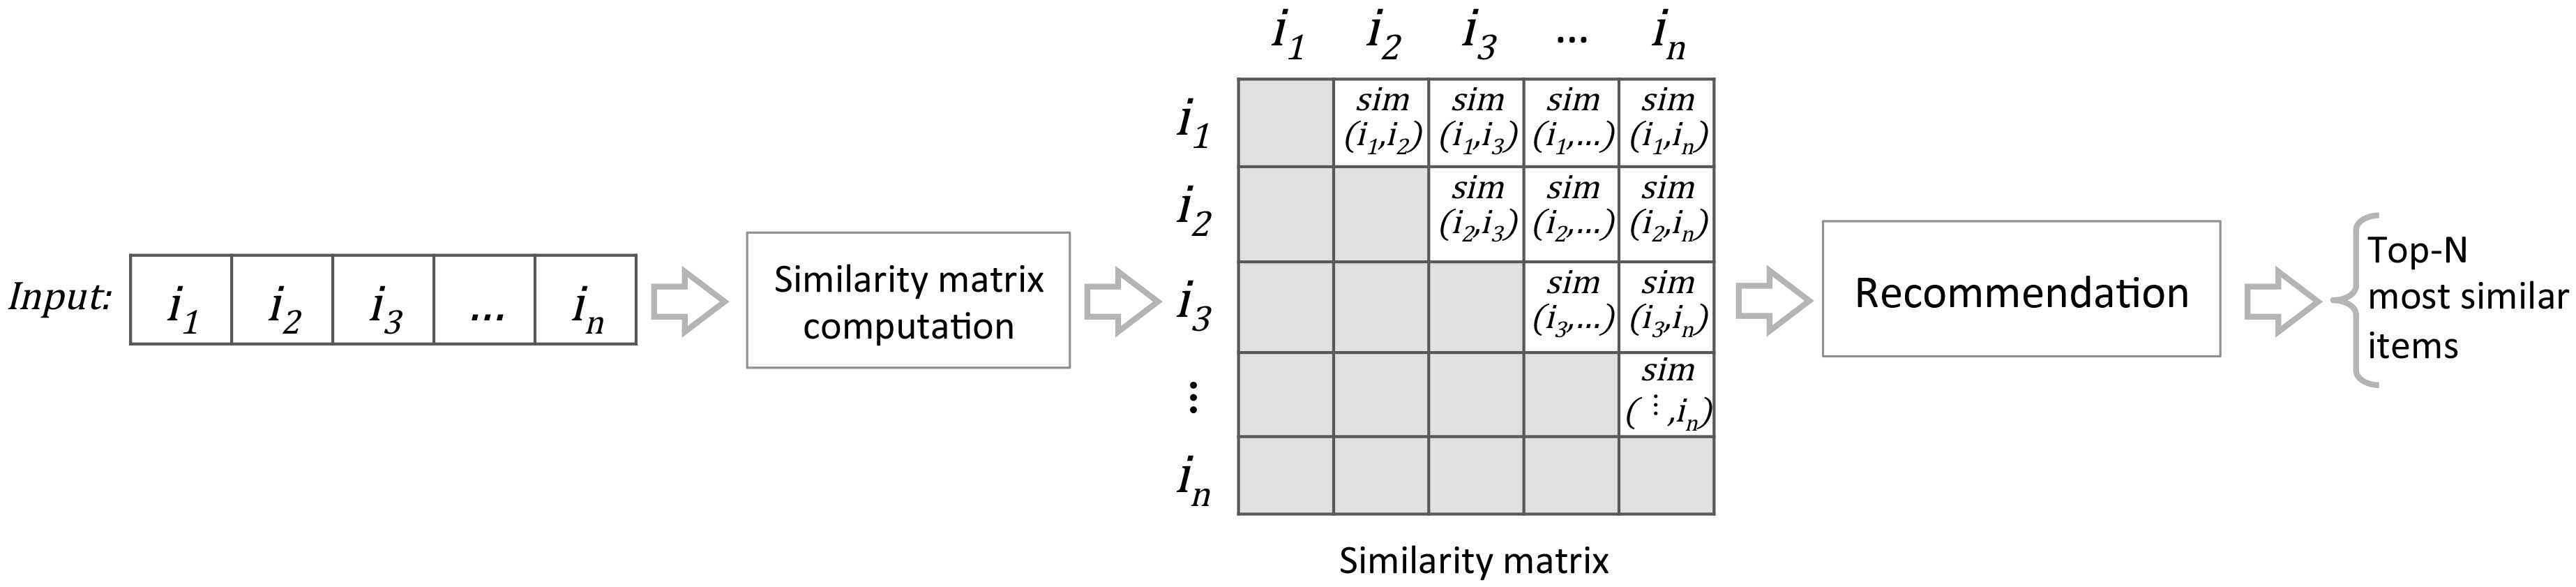
\includegraphics[width=12cm]{./images/flows/flow_content_based_filtering_diagram.jpg}
   \caption{The Content-Based Filtering process. Creation of the similarity matrix and computation of the top most similar items.}
   \label{fig:itemBasedProcess}
\end{figure}
\\
For instance, the Pandora Radio~\cite{pandoraInternetradio} uses a subset of approximately 400 different song characteristics in order to recommend the "radio station" that plays music with similar properties to that preferred by the user. On the other hand, user's feedback is used to adjust the algorithm whenever one likes or dislikes some music~\cite{recommenderSystemWiki}.\\
\\
For the current problem of a tourist guide development, in order to use, integrate, and adopt \gls{cbf} algorithms in our work, we could use a large set of attributes to characterize points of interest, such as the landscape, urban, nature, mountain, monument, and so on. Figure~\ref{fig:exampleCBF} illustrates an example of a \gls{cbf} recommender system with one user and three distinct locations.\\
\\
\begin{figure}[h!]
 \centering
   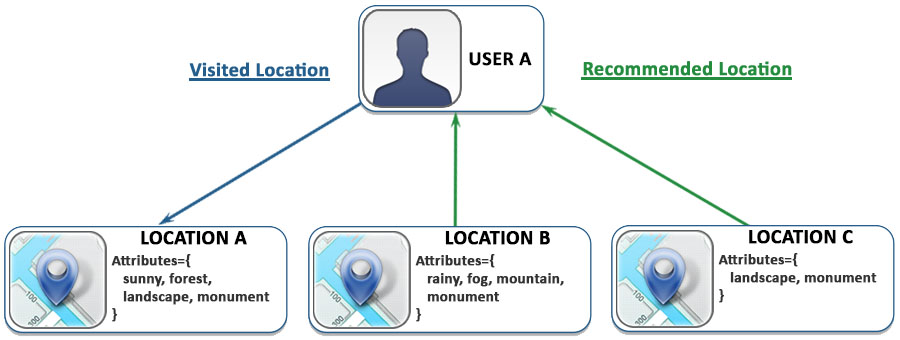
\includegraphics[width=12 cm]{./images/examples/example_content_based_filtering.jpg}
   \caption{Example of a recommender system process using a \gls{cbf} approach.}
   \label{fig:exampleCBF}
\end{figure}
\\
Assuming that \verb"User A" visits the \verb"Location A", that same user will receive a recommendation to both \verb"Location B" and \verb"Location C" since it shares the same attribute \verb"Landscape" and \verb"Monument" with the visited location. For the current problem, it is possible to find a lot of attributes that will characterize the point of interest. A possible problem lies in the human factor. It is that users have the possibility to insert new locations. The recommender system may have a negative impact by suggesting wrong locations when users make a mistake on the attribute definition during the location creation phase.\\
\\
Figure~\ref{fig:exampleALgCBF} shows an example of the \gls{cbf} algorithm which refers to the information represented in Figure~\ref{fig:exampleCBF}.
%%%%%%
\begin{figure}[h!]
 \centering
   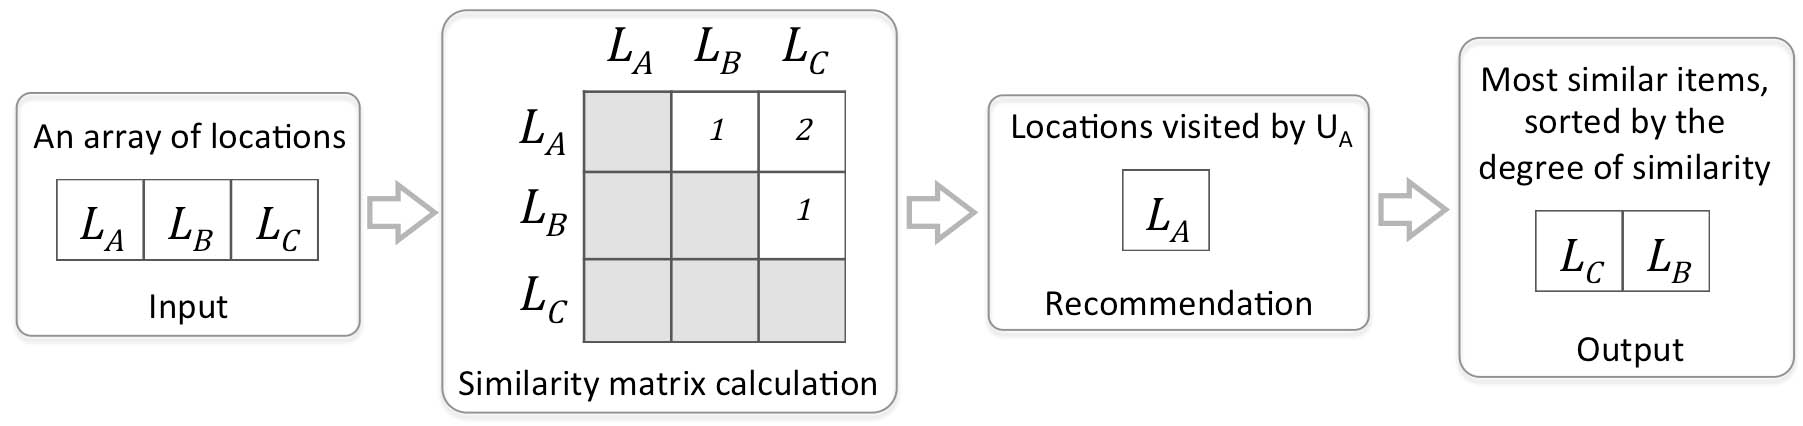
\includegraphics[width=14.5 cm]{./images/flows/flow_example_diagram_cbf.jpg}
   \caption{The \gls{cbf} approach sequence. The computation of the similar items is illustrated for 3 items.}
   \label{fig:exampleALgCBF}
\end{figure}
As input we have an array of locations, which is used to compute a similarity matrix in order to measure the degree of similarity between those items. We compute $sim(L_{A},L_{B})=1$, $sim(L_{A},L_{C})=2$ and $sim(L_{B},L_{C})=1$. Later, during the recommendation phase, we exclude the locations visited by the user from the resulting set. The produced output is an array of locations sorted in decreasing order by their degree of similarity.

\section{Overview of Collaborative Filtering}
\label{sec:ocft}

In this Section, we introduce \gls{cf} algorithms, with an analysis of the recommendation process. The goal of a \gls{cf} algorithm is to suggest new items for a particular user based on user's previous opinions and the opinions of other users with similar taste~\cite{ibCollabrativeVSGK}. We first introduce a  generic definition of a \gls{cf} algorithm, what kind of data is used as input and output as well as a definition of the data transformation process.\\
\\
%%%%%%%%%%%%%%%
As mentioned previously, the~\gls{cf} approach is divided in two types: Model-Based and Memory-Based. Memory-Based algorithm utilizes user rating data to compute similarity between users or items while the Model-Based uses data mining and machine learning algorithms to find patterns based on training data. As shown in Figure~\ref{fig:cfProcess}, the algorithm has as input an entire user-item matrix $m \times n$
of users $U = \{u_{1}, u_{2}, \dots , u_{j}, \dots u_{m}\}$ 
by items $I = \{i_{1}, i_{2}, \dots , i_{j}, \dots,  i_{n}\}$. Each entry $a_{i,j}$ in the user-item matrix represents the preference score in a numerical scale of the $i$th user on the $j$th item. The \emph{recommendation} part of the algorithm has as output a list of the most similar items for the active user $u_{a}$. The \emph{prediction} part of the algorithm produces the prediction $P_{a,j}$ for the specific item $i_{j}$ for the active user $u_{a}$, which expresses the predicted likeness of item $i_{j} \notin I_{u_{a}}$ for $u_{a}$, where $I_{u_{a}}$ is a set of items that belong to $u_{a}$.
\begin{figure}[h!]
 \centering
   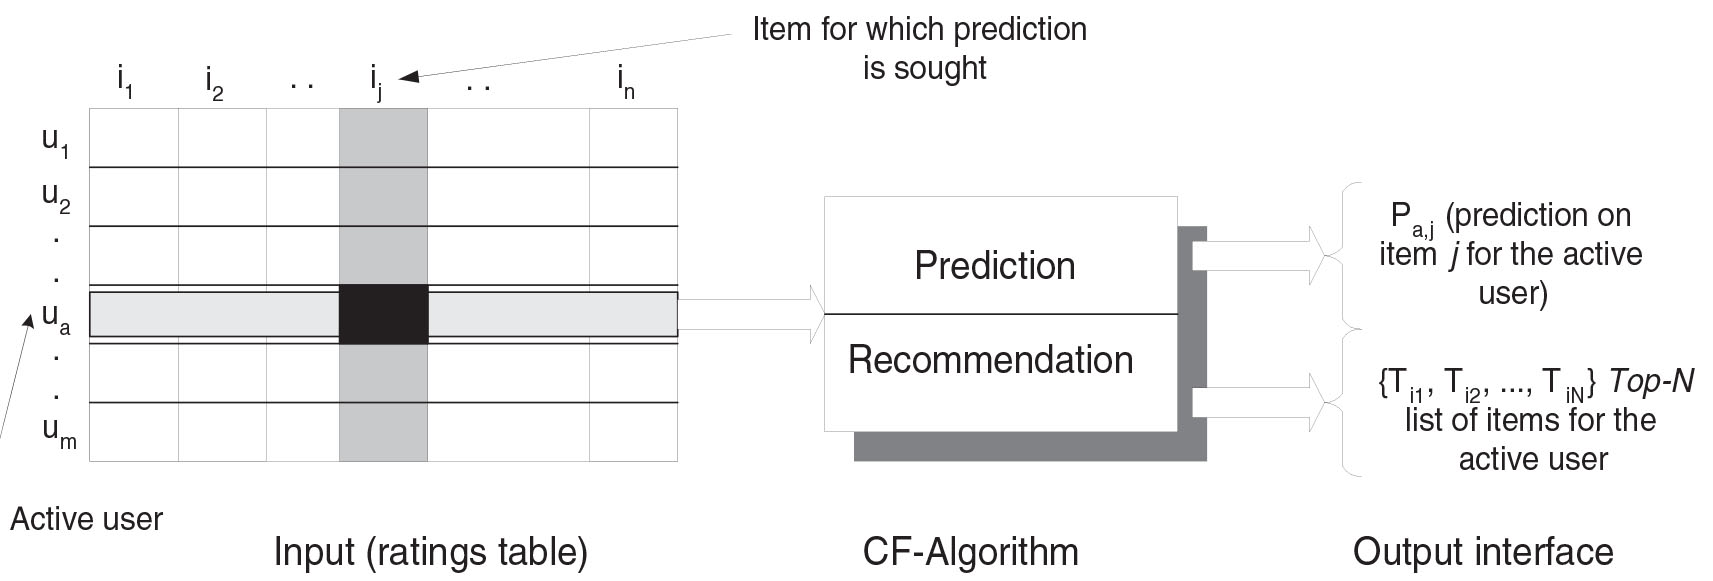
\includegraphics[width=14.5 cm]{./images/flows/flow_cf_algorithm_process.jpg}
   \caption{The Collaborative Filtering Process (adapted from~\cite{ibCollabrativeVSGK}). }
   \label{fig:cfProcess}
\end{figure}
\\
In order to integrate this type of algorithms into this project, each item will be a point of interest. The~\gls{cf} algorithm will be used to suggest locations for each user, providing an output containing the following characteristics:
\begin{itemize}
 \item A list of locations that have not been visited by the user;
 \item The list depends on the user's past visits.
\end{itemize}
Figure~\ref{fig:exampleIBF} shows an example of a \gls{cf} recommender system. As the recommendation process is based on the user's past actions, \verb"User A" has visited \verb"Location A" and \verb"Location C" while \verb"User B" has only visited \verb"Location C". The system will determine that \verb"User A" and \verb"User B" have similar preferences since they both have visited \verb"Location C" and then it will recommend \verb"Location A" to \verb"User B".\\
\begin{figure}[h!]
 \centering
   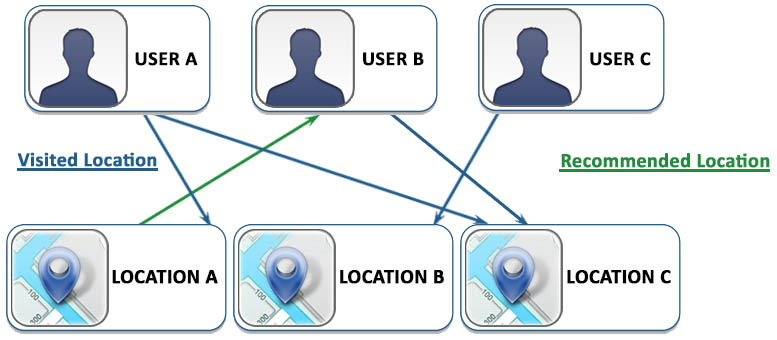
\includegraphics[width=12 cm]{./images/examples/example_item_based_filtering.jpg}
   \caption{Example of a recommender system using a \gls{cf} approach.}
   \label{fig:exampleIBF}
\end{figure}

\subsection{User-Based Approach}
\label{subsec:userBasedCF}
This Section describes the User-Based Collaborative Filtering (UBCF) methodology with Memory-based algorithms. The purpose of this category of algorithms is introduced along with their benefits and disadvantages.\\
\\
The Memory-Based approach uses statistical analysis methods to find a set of users, designated by neighbors, that have similar preferences. It searches for neighbor users with a large number of preferences in common. The most commonly used algorithms are the \gls{knn}~\cite{Aha91}\cite{Duda_Book} and the \gls{lsh}~\cite{neighborhoodCF}.\\
\\
%\marginpar{} %%%
The \gls{knn} algorithm consists in finding the top K nearest neighbours for an item. Unknown ratings are predicted from a list of nearest neighbors which involve finding the user-to-user or item-to-item correlations. For large datasets, this algorithm imposes a significant computational burden.\\
\\
In the presence of a wide range of users and items, the preferred algorithm would be \gls{lsh}. It implements the nearest-neighbor mechanism in linear time and does not consider the content of the recommended items. The~\gls{lsh} algorithm is more effective on large data sets when an appropriate hash function is chosen~\cite{googleScalableCF}, but its performance decreases when data gets sparse~\cite{ibCollabrativeVSGK}.

\subsection{Item-Based Collaborative Filtering}

This Section details the Item-Based Collaborative Filtering (IBCF) with Model-based methodology for producing predictions to users. This type of algorithms follows a different approach, as compared with user-based algorithms, from Subsection~\ref{subsec:userBasedCF}. Item-based approach looks into a set of items that a specific user has rated and computes a set of similar $k$ items $\{{i_{1}, i_{2}, \dots , i_{k}\}}$, as well as the similarities between themselves $\{{s_{i1}, s_{i2}, \dots , s_{ik}\}}$. \\
\\
The Model-Based method provides recommendation for items after defining a model based on user classifications. This type of algorithm uses data mining and machine learning techniques and offers some benefits regarding scalability as compared with the Memory-Based model. Usually the model building process is performed by algorithms such as Bayesian Networks~\cite{Bayesian} and rule-based approaches~\cite{ibCollabrativeVSGK}. The Bayesian network model formulates a probabilistic model for the \gls{cf} problems. The rule-based approach applies association rule discovery algorithms to find association between co-purchased\footnote{This example refers to e-commerce, but it can be applied in almost any scenario.} items and then generates item recommendations based on the strength of the association between items~\cite{ibCollabrativeVSGK}.\\
\\
%%%%%%%%%%%%%
This type of algorithms handles data sparsity and scalability without negative implications on prediction. The disadvantage of this approach lies in the model building process. Large models should be considered in order to have good predictions but exhibit negative implications on both performance and scalability. By reducing the model size, loss of useful information may occur which worsens the quality of the predictions. One needs to have a tradeoff between scalability and prediction performance. Item-based~\gls{cf} generates predictions by using the user's own ratings for other items combined with those similarities to the target item, rather than other users' ratings and user similarities as in User-based~\gls{cf}. A \gls{rs} needs a similarity function and a method to generate predictions from ratings and similarities~\cite{cfrsBook}.\\
\\
In our system, each user will have the possibility to rate the visited locations in order to express the degree of enjoyment during the visit. Through collaboration of various users, the collected data will be used to compute the average rating for each location and later recommend it to users that haven't visited it yet. Figure~\ref{fig:ibcfProcessStep1} illustrates the first step of the recommendation process. It consists in the calculation of the item-to-item similarity matrix, which will compute the related pairs as $sim_{i,j}$. 
\begin{figure}[h!]
 \centering
   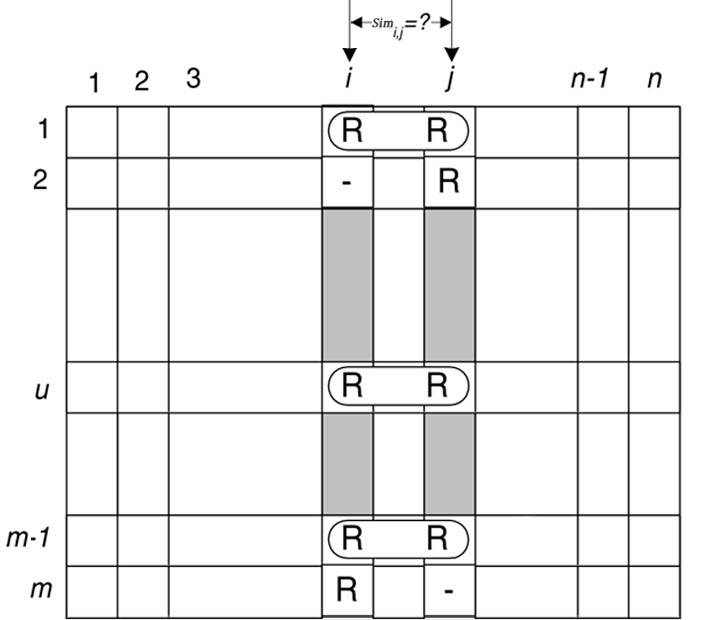
\includegraphics[height=5.0cm]{./images/flows/flow_item_based_filtering_1.jpg}
   \caption{Isolation of the items with same rating value (Adapted from~\cite{ibCollabrativeVSGK}).}
   \label{fig:ibcfProcessStep1}
\end{figure}\\
The next step of the recommendation process, illustrated in Figure~\ref{fig:ibcfProcessStep2}, consists in producing the list of the recommended items. The output of the algorithm is a set of items sorted by the similarity ranking to the $i$-th item. After isolating the most similar items based on the similarity measures, the next step is to look into the target users ratings and obtain a prediction of the most similar items~\cite{ibCollabrativeVSGK}.
\begin{figure}[h!]
 \centering
   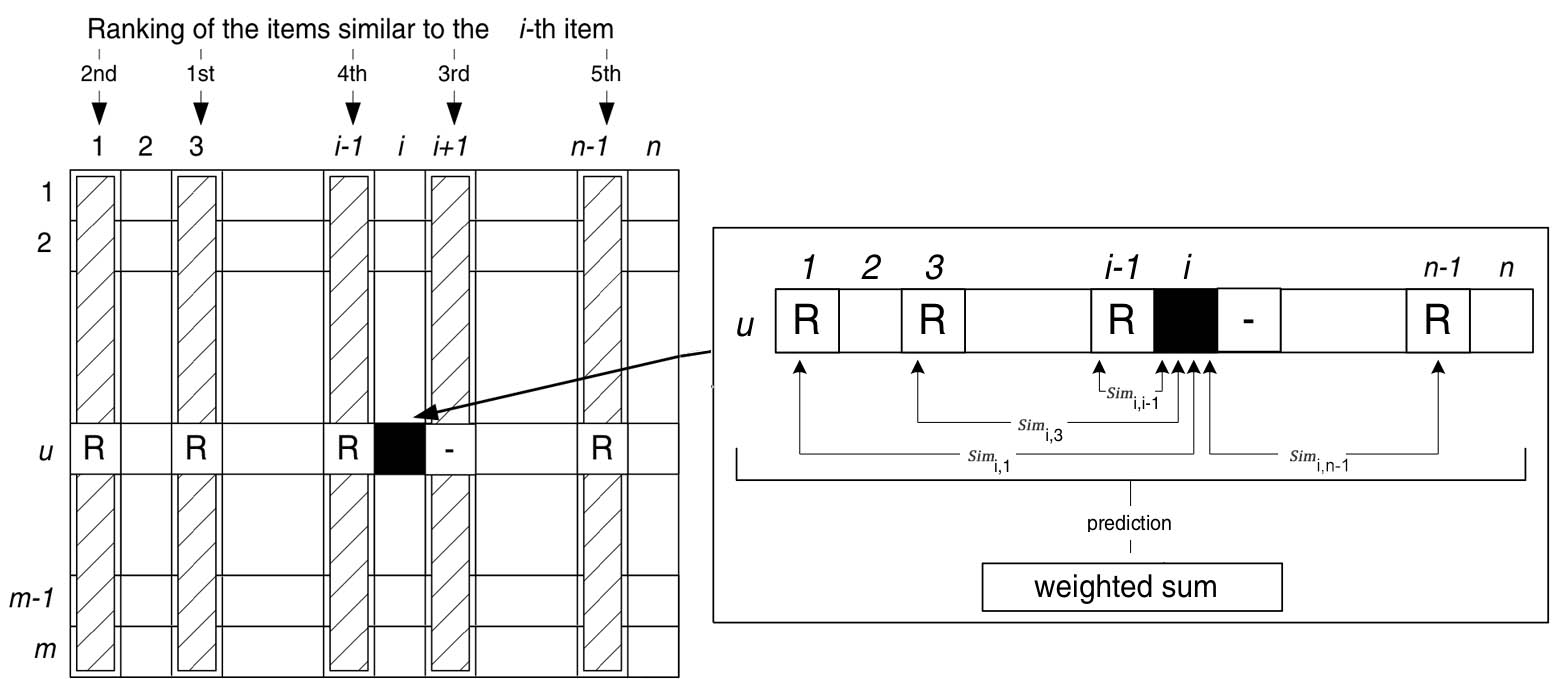
\includegraphics[height=5.0cm]{./images/flows/flow_item_based_filtering_2.jpg}
   \caption{The Item-Based Collaborative Filtering Process with prediction generation process (Adapted from~\cite{ibCollabrativeVSGK}).}
   \label{fig:ibcfProcessStep2}
\end{figure}\\
\\
%%%%%%%%%%%%
There are many different ways to compute the similarity between items. The most commonly used methods are the Adjusted Cosine Similarity, Cosine based Similarity, and Correlation based Similarity~\cite{ibCollabrativeVSGK}. After obtaining the similarities between items, the next step is to generate the output interface in terms of prediction. The prediction computation is obtained by looking into target user's ratings and use a weighted sum to obtain predictions. The aim of this technique is to compute prediction on item $i$ for user $u$ by computing the sum of ratings given by user $u$ on the items similar to $i$. Items $i$ and $j$ are weighted by corresponding similarity $sim_{i,j}$~\cite{ibCollabrativeVSGK}.\\
\\
An example illustrating how the recommendation process works with this type of algorithms is shown in Figure~\ref{fig:ibcfExample1}.
\begin{figure}[h!]
 \centering
   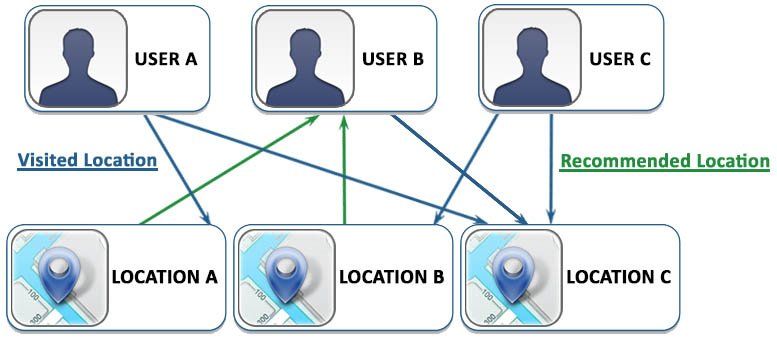
\includegraphics[width=11 cm]{./images/examples/example_item_based_filtering2.jpg}
   \caption{The Item-Based Collaborative Filtering example.}
   \label{fig:ibcfExample1}
\end{figure}
We consider that the three users have visited \verb"Location C" and have rated equally each one of the visited locations. The similarity is computed by first obtaining the list of users that have visited the location in cause. Then, for each one of those users, a list of locations that share the same rating as the targeted location is retrieved. The algorithm will recommend both \verb"Location A" and \verb"Location B" to \verb"User B", since those are considered similar by \verb"User's B" actions.\\
\\
An example of the \gls{ibcf} algorithm is presented in Figure~\ref{fig:exampleAlgIBCF}. In order to simplify the following examples, \verb"User B" is denoted as $U_{B}$, \verb"Location A" as $L_{A}$, \verb"Location B" as $L_{B}$, and so on.\\
\\
\begin{figure}[h!]
 \centering
   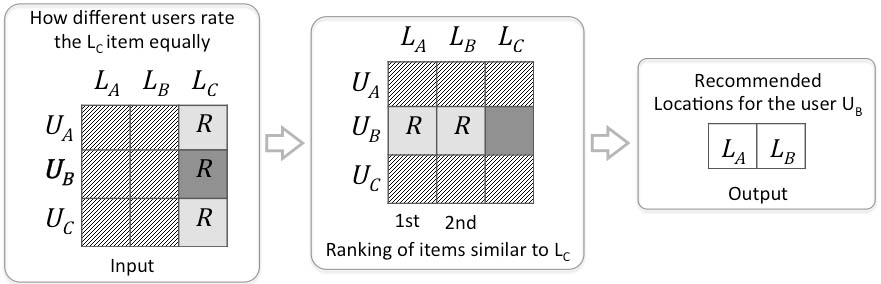
\includegraphics[width=11 cm]{./images/flows/flow_example_diagram_ibf.jpg}
   \caption{An algorithm example of the \gls{ibcf} approach.}
   \label{fig:exampleAlgIBCF}
\end{figure}
\\
In this example, we compute locations similar to $L_{C}$ for the active user $U_{B}$. Considering that $U_{B}$ has rated $L_{C}$ with the rating $R$, we search for other users that have rated the same location equally. From these users, we retrieve a set of locations that share the same rating value $R$ but weren't visited by $U_{B}$, in this case $L_{A}$ and $L_{B}$. Then, we rank those by computing the weighted sum for the ratings. The algorithm produces a sorted array of locations, namely $L_{A}$ and $L_{B}$.

\section{Algorithm Comparison}
\label{sec:cbtda}

In order to compare the approaches reviewed in this Section, the following set of characteristics was chosen:
\begin{itemize}
\item \textbf{Easy Implementation} - Refers to the complexity of the algorithm implementation.
\item \textbf{Scalability} - Describes the algorithm ability to handle an increasing amount of data without noticeable performance implications.
\item \textbf{Performance} - Refers to a reasonable algorithm performance without introducing a large computational burden in the system.
\item \textbf{Data Sparsity} - Users tend to rate only a few items over the entire set, resulting in a very sparse matrix\footnote{A sparse matrix has many entries set to zero.}. The computed matrix doesn't have useful rating information which degrades the algorithm performance, producing poor recommendations.
\item \textbf{Cold Start} - Also known as the first rater problem. Caused by the data sparsity. Refers to the lack of information related to the new users which does not have past preferences. The system cannot draw any inferences for users or items about which it has not yet gathered sufficient information. New users will need to rate a sufficient number of items to ensure that the system provides reliable recommendations for them.
\item \textbf{Grey-Sheep problem} - Refers to a set of users that have low correlation coefficients with other users, as they partially agree or disagree with other users. The presence of these users in a small community may result in inaccurate recommendations for those users. Larger communities of these users may negatively affect the overall recommendations of the system.
\end{itemize}
Table~\ref{tab:filterComparison} lists a comparison of the advantages and disadvantages of the filtering approaches, discussed in this Section.
\begin{center}
\begin{table}
	\centering
    \caption{Comparison of various filtering approaches.}
    \label{tab:filterComparison}
    \begin{tabular}{c}
	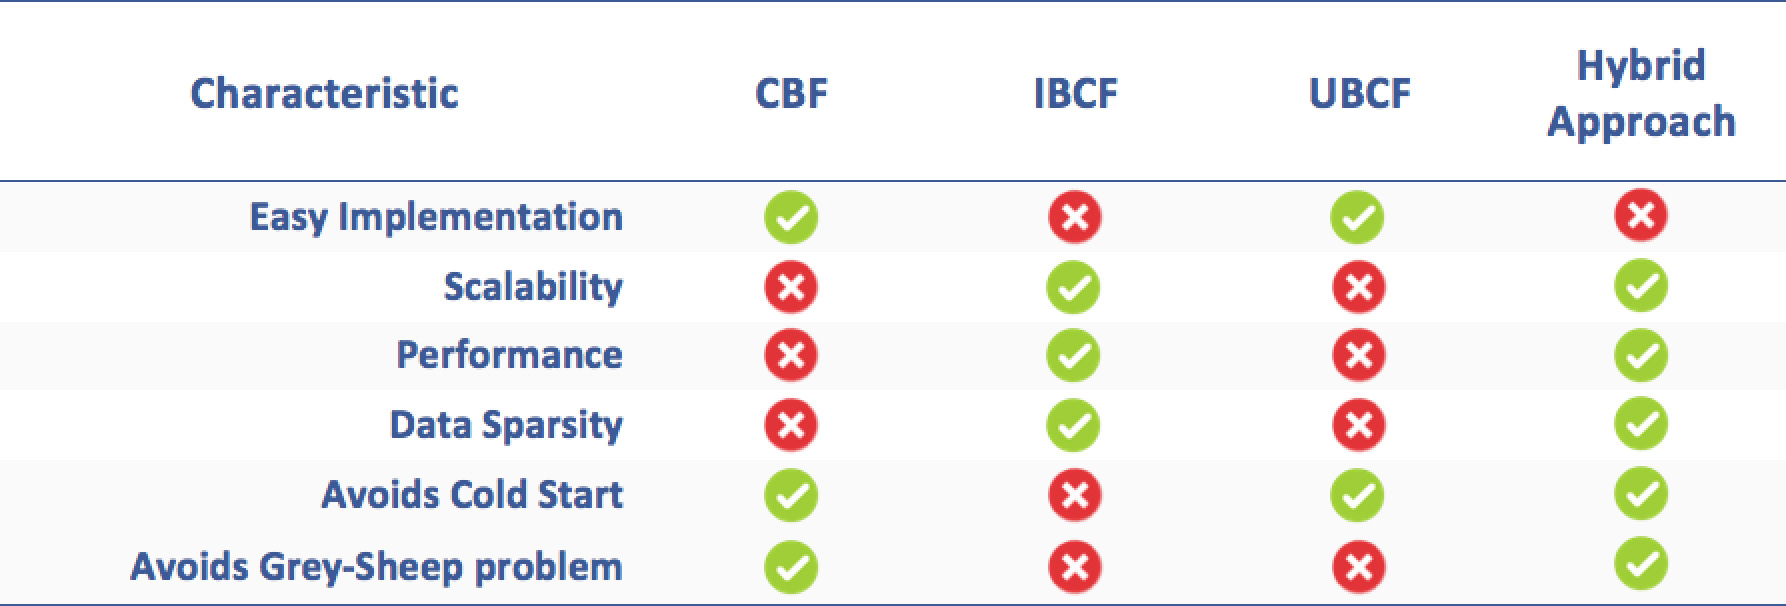
\includegraphics[width=13cm]{./images/tables/table_filter_comparison.jpg}    
    \end{tabular}
    \end{table}
\end{center}
%%%%%%%%
\gls{cbf} recommender systems, computes correlations between the content of the items and the user's preferences as opposed to \gls{ubcf} or \gls{ibcf} systems that choose correlation between users or items with similar preferences~\cite{content-based-Filtering}. The~\gls{cbf} algorithms are simple to implement and if the item attributes are correctly selected, they can improve their performance~\cite{CBFandCFApproach}, but not on a large scale. Because of inaccurate predictions, this type of algorithms is not appropriate for the current problem of a tourist guide. The \gls{cf} technique is a preferable choice when compared with the~\gls{cbf}, namely the \gls{ubcf} and \gls{ibcf} approaches, which have presented more benefits and are more accurate in terms of predictions, thus excluding~\gls{cbf} as the candidate for the implementation of the \gls{rs} in this project. Although the \gls{cf} technique is better than the \gls{cbf} technique in some aspects, it is worse in other aspects, as pointed in Table~\ref{tab:filterComparison}. So, researchers have recently developed hybrid approaches that overcome deficiencies of both systems acting in isolation. Despite the fact that in the~\gls{rs} literature, the use of a hybrid approach is usually preferable~\cite{rsHybridApproach} as compared to other approaches, we choose to use in our work the IBCF approach.\\
\\
Through the research that was made, we conclude that IBCF approach presents sufficient amount of benefits for our scenario. While hybrid approaches are better, they were considered very complex to be implemented in the available time. The complexity of the IBCF RS is lower, it handles appropriately the information from our service while making accurate recommendations, thus being our first choice for the RS. The main disadvantages of the IBCF approach (described in Table~\ref{tab:filterComparison}) are its complexity, the cold start, and the grey-sheep problems. In the current project, the complexity problem is contoured by using the Mahout~\cite{apacheMahout} framework, which provides a robust implementation of varied RS with support to different algorithms, including those described in this document. Neither the cold start nor gray-sheep problems were addressed in this project.\\
\\
Moreover, the experimental results detailed in Subsection~\ref{subsec:expRsults} helped us to choose
the Slope One~\cite{slopeOne} algorithm, which fits best in our scenario. The Slope One algorithm has shown more benefits when compared with other solutions, namely in performance, variation of the model size, recommendation quality, among others.\\
\\
The Slope One algorithm is a family of algorithms used for~\gls{cf}. It assumes that there's some linear regression between the rating value of one item and another. The estimated preference $Y$ is given by the equation
\begin{equation}
Y = mX + b,
\end{equation}
with $m=1$, and $X$ representing the item on which the preference is based. The average difference in the preference value for every pair of items is represented by $b$.\\
\\
The algorithm handles computations quickly, providing a good performance. As all the information is stored in memory, the large amount of item-item preference value differences can cause memory issues~\cite{mahoutInAction}. Suppose that we have $n$ items, $m$ users. Computing the average rating differences for each pair of items requires a matrix with up to $n(n-1)/2$ entries, and up to $mn^2$ time steps~\cite{slopeOneComplexity}.
%%%%%%%%
%%%%%%%%
\section{Slope One - Hand Calculations}
\label{sec:slopeOneHandCalculations}
In this Subsection, we describe the pseudo-code of the Slope One algorithm, as also we manually compute a set of recommendations for a chosen example, to illustrate each step of the algorithm chosen for our recommender system~\cite{mahoutInAction}.\\
\\
The algorithm is divided in two stages: pre-processing and recommendation. Algorithm~1 describes the pseudo-code of the pre-processing stage of the Slope One deviation matrix~\cite{slopeOneWeighted}.\\
\begin{algorithm}[h!]
\label{alg:SlopeOneMatrix}
\begin{algorithmic}[1]
{\small
\caption{Computation of Slope One deviation matrix.}
	\REQUIRE \hspace{.2cm} $U$: set of all users.\\
 	\indent \hspace{.8cm}  $S$: set of all items.\\
	\indent \hspace{.8cm}  $R$: set of all rated items.\\
	\ENSURE $dev$: deviation matrix.\\
	\indent \hspace{.7cm} $freq$: co-rating frequency matrix.\\
	\vspace{1mm} \hrule \vspace{1mm}	\small
	/* Step 1 */
	\FOR {$all~u \in U$}
	  	\FOR {$all~i \in Ru$}
			\FOR {$all~j \in Ru$}
				\STATE $dev_{[i,j]} \leftarrow dev_{[i,j]} + (r_{[u,i]} - r_{[u,j]})$
				\STATE $freq_{[i,j]} \leftarrow freq_{[i,j]} + 1$
			\ENDFOR	
		\ENDFOR	
	\ENDFOR		
	\\
	/* Step 2 */
	\\
	\FOR {$all~i \in S$}
	  	\FOR {$all~j \in S$}
	  		\STATE $dev_{[i,j]} \leftarrow \frac{dev_{[i,j]}}{freq_{[i,j]}}$
		\ENDFOR	
	\ENDFOR				
}
\end{algorithmic}
\end{algorithm}\\
%%%%%%
On Table~\ref{tab:handCalcStep1} we present the input data that is used to perform the hand calculations. The input dataset contains 4 users and 4 touristic locations, where some of these locations were not rated by all users.
%%%%%%
\begin{center}
\begin{table}
	\centering
    \caption{The input dataset used by the hand calculations.}
    \label{tab:handCalcStep1}
    \begin{tabular}{c}
	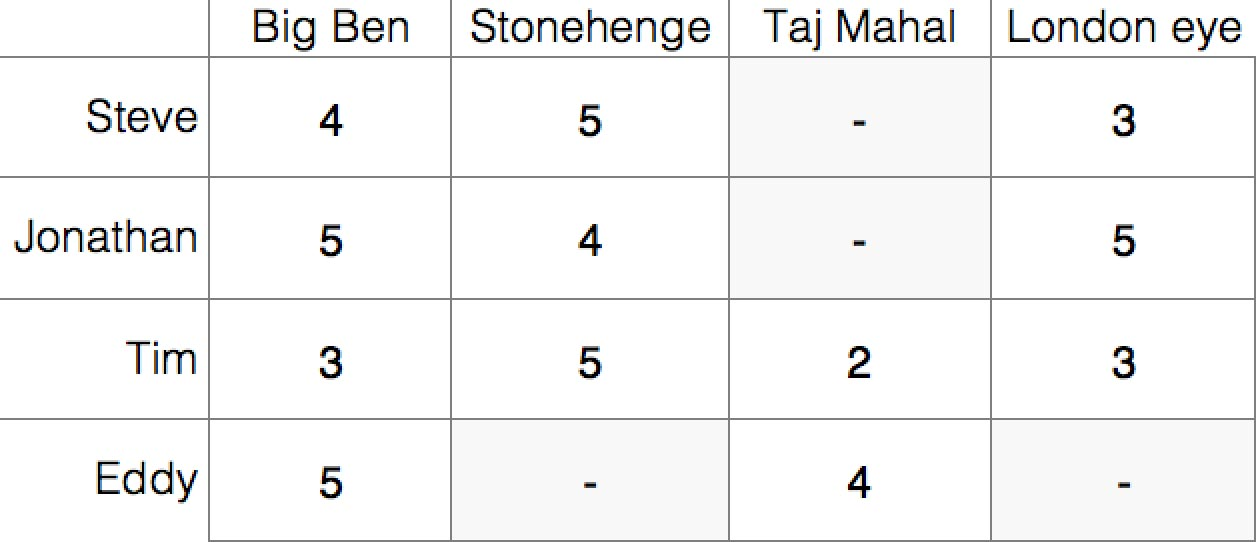
\includegraphics[width=7cm]{./images/tables/table_slope_one_step_by_step_step_1.jpg}    
    \end{tabular}
    \end{table}
\end{center}
%%%%%%
On Table~\ref{tab:handCalcStep2} we compute the entries for the deviation matrix through \emph{Step 1} of the algorithm (Algorithm~1). For each rated pair of items, we add the difference between the items $i$ and $j$ to the already existing value for index $[i,j]$ in $dev$. In this phase, we also increment the value of $freq$ for each difference between $i$ and $j$.\\
%%%%%%
\begin{center}
\begin{table}
	\centering
    \caption{Calculation of the entries for the deviation matrix.}
    \label{tab:handCalcStep2}
    \begin{tabular}{c}
	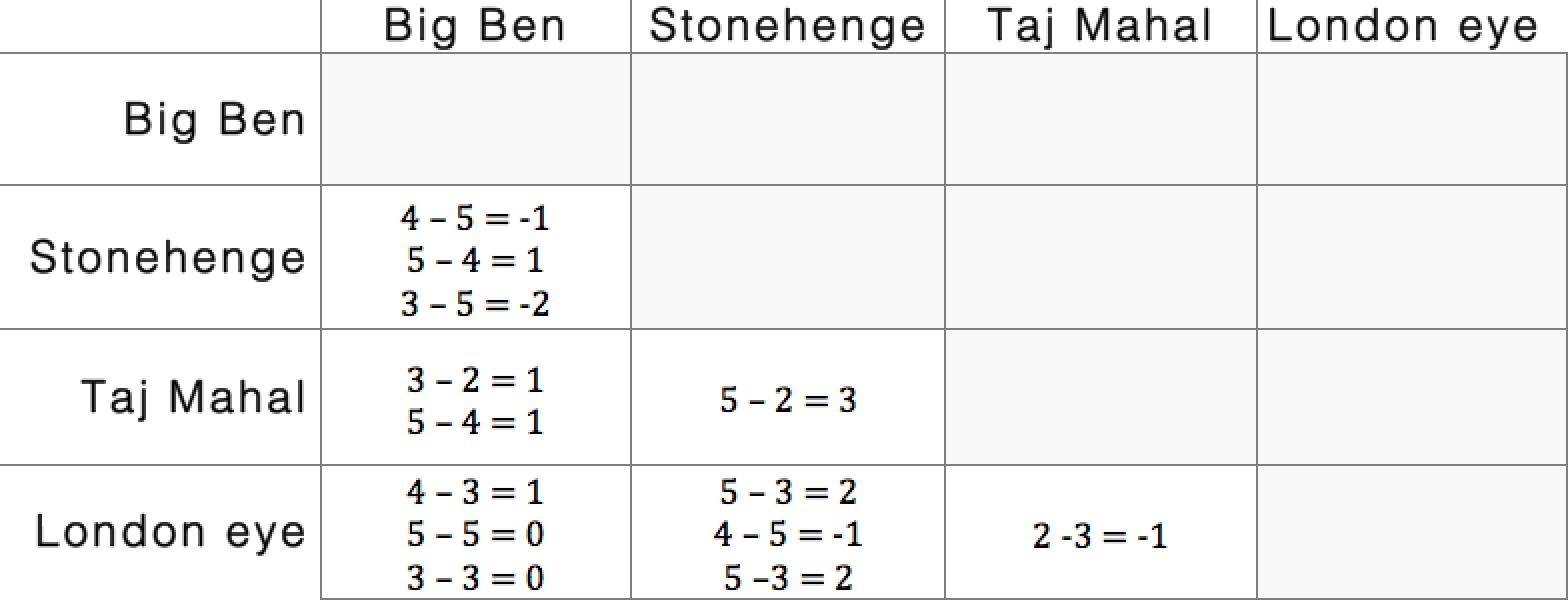
\includegraphics[width=8cm]{./images/tables/table_slope_one_step_by_step_step_2.jpg}    
    \end{tabular}
    \end{table}
\end{center}
%%%%%%
The result of the \emph{Step 2} (Algorithm~1) is described on Table~\ref{tab:handCalcStep3}, which iterates through the $dev$ matrix. For every index $[i,j]$ we calculate the average of the value stored in that index by dividing the sum of each component by the $freq$ value of the corresponding index.\\
\begin{center}
\begin{table}
	\centering
    \caption{Deviation matrix with average difference between each combination of items.}
    \label{tab:handCalcStep3}
    \begin{tabular}{c}
	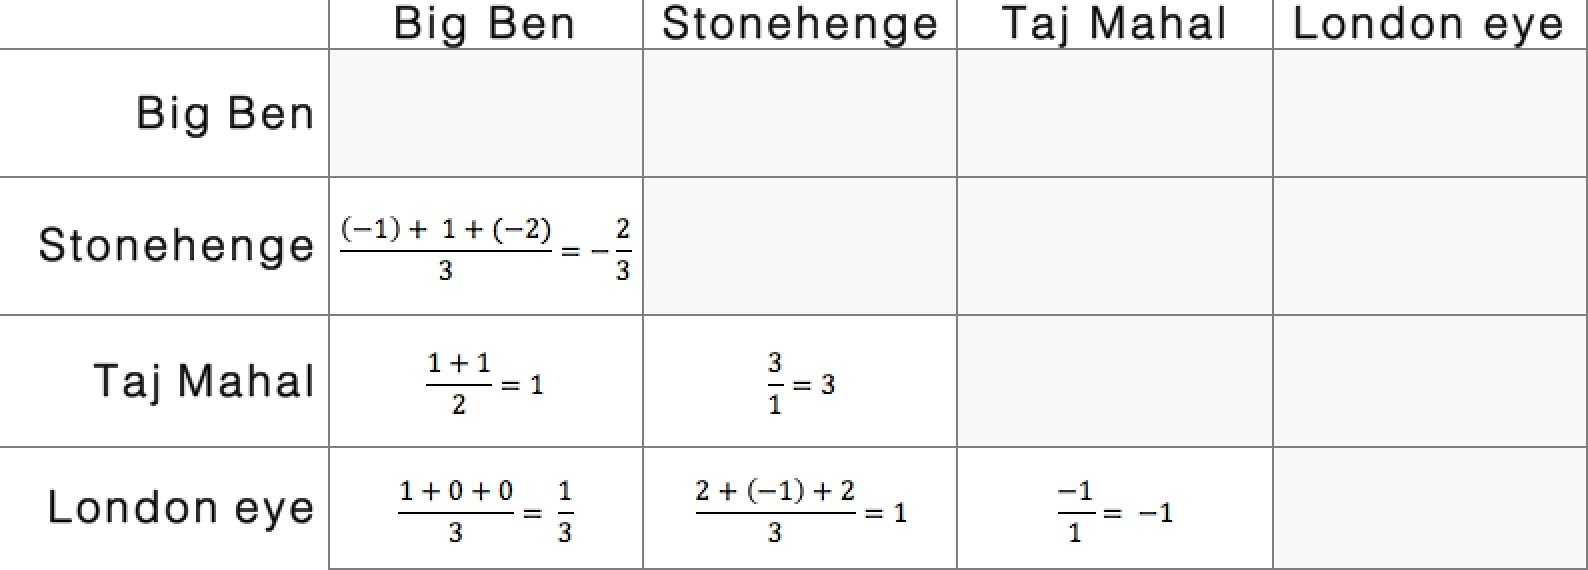
\includegraphics[width=8cm]{./images/tables/table_slope_one_step_by_step_step_3.jpg}    
    \end{tabular}
    \end{table}
\end{center}
The final $dev$ matrix contains the average difference between each combination of items. For example, the difference value for the \verb"Stonehenge" and \verb"Taj Mahal" is 3.0, which means that, on average, the item \verb"Stonehenge" is rated above the item \verb"Taj Mahal" by 3.0.\\
\\
Now we will apply the calculations required by the recommendation stage, which will have as output a list of recommendations computed for user \verb"Eddy". The following format is used to specify the involved components:\\ 
$R_{\{User~that~receives~recommendation, Recommended~location, Base~location~used~for~the~rating~computation\}}$.\\
\\
$R_{\{Eddy, Stonehenge, Big Ben\}} = 5 + (-\frac{1}{2}) = 4.5$\\
$R_{\{Eddy, Stonehenge, Taj Mahal\}} = 4 + 3 = 7$\\
$R_{\{Eddy, Stonehenge\}} = \frac{3 * 4.5 + 1 * 7}{3 + 1} = 5.125$\\
\\
$R_{\{Eddy, London Eye, Big Ben\}} = 5 + \frac{1}{2} = 5.5$\\
$R_{\{Eddy, London Eye, Taj Mahal\}} = 4 + (-1) = 3$\\
$R_{\{Eddy, London Eye\}} = \frac{3 * 5.5 + 1 * 3}{3 + 1} = 4.875$\\
\\
For user \verb"Eddy", the recommendation list will have two entries sorted in decreasing order by the estimated value: [5.125 - \verb"Stonehenge", 4.875 - \verb"London Eye"].

%%%%%%%%
%%%%%%%%
\section{RS Application in Tourist Guidance}
\label{sec:rsInTouristGuides}
As of time of this writing (November 2013), \gls{rs} are being integrated in almost every scenario where these can help users to discover new useful information. In tourist guide scenario, with integration of the \gls{rs}, users can become their own travel agents. The recommended touristic locations match user's preference to provide reliable recommendations which can be accessed at any time and anywhere.\\
\\
Applications such as TouristEye and Foursquare already implement the \gls{rs} with \gls{cf} approach~\cite{foursqureRecommendationEngine}~\cite{tourisEyeRecommender}. These services provide users with the touristic locations that they might like to visit, based on their preferences. The developers of these solutions did not provided any detailed information regarding the \gls{rs} that powers their service.\\
\\
The chosen \gls{cf} approach for the GuideMe project has demonstrated to provide accurate results. Combined with the Slope One algorithm, it provides fast and reliable recommendations of the touristic locations, and handles well the sparsity of users’ ratings, improving the quality of the recommendation system~\cite{itemBasedSlopeOne}.\\
\\
There are some studies focused on the efficiency, complexity and reliability of the artificial intelligence-based architectures for the~\gls{rs} component. This architecture is based on several machine learning techniques, such as linear models, neural networks, classification and text mining~\cite{intelligenHybrid}. The combination of these techniques contributes positively to the overall quality of the~\gls{rs}.